\subsection{Initializing the Directed Graph}
In the original Opioid Spread Model, we temporarily overlooked the relationship between the parameter $\lambda$ and position $(x,y)$ in the formula. In this section, we modify our model to reveal the relationship between $\lambda$ and local socio-economic factors. 

Similar to the method introduced in 4.3-4.4, we define Main Source as counties ranked first-level Sources for more than 4 years among 2010-2017. We discovered the following seven Main Sources for General Opioids.

\begin{table}[H]
	\centering
	\begin{tabular}{|c|c|c||c|c|c|}
		\hline
		\rowcolor[HTML]{656565} 
		{\color[HTML]{FFFFFF} \textbf{STATE}} & {\color[HTML]{FFFFFF} \textbf{COUNTY}} & {\color[HTML]{FFFFFF} \textbf{F}} &{\color[HTML]{FFFFFF} \textbf{STATE}} & {\color[HTML]{FFFFFF} \textbf{COUNTY}} & {\color[HTML]{FFFFFF} \textbf{F}}\\ \hline
		KY & - & - &OH & Mahoning & 2115 \\ \hline
		VA & - & - &OH & Cuyahoga & 12190\\ \hline
		WV & - & - &OH& Lake &3003 \\ \hline
		OH & Hamilton & 11896 &PA & Philadelphia & 23431 \\ \hline
		OH & Stark & 2539 & PA & Allegheny & 8268 \\ \hline
	\end{tabular}
	\centering
	\caption{Main Sources of Opioids in General}
\end{table}

Since detailed information concerning opioid amount is limited, and the properties of $\lambda$ differ regarding whether the county is a Source or a Consumer , we need to make the following assumptions to simplify our model in order to estimate the value of $\lambda$:

\begin{enumerate}
	\item For Consumers, $\lambda \approx 1$. This indicates that Consumers have a limited ability to transport drugs into neighboring counties, and can be omitted when conducting simplified calculations.
	
	\item Based on the above assumption, we can estimate $\lambda$ for Sources by
	\begin{equation}
	\lambda_{Source_i}=\frac{F_{Source_i}}{F_{Source_i}+\sum_{j\in N_i} F_{Consumer_j}}
	\end{equation} 
\end{enumerate}

\textit{
NOTE: In the following analysis, we abbreviate $\lambda_{Source_i}$ to $\lambda_i$, since we will mainly be considering the $\lambda$ value for Sources, and therefore no confusion shall occur. 
}

\begin{figure}[H]
	\centering
	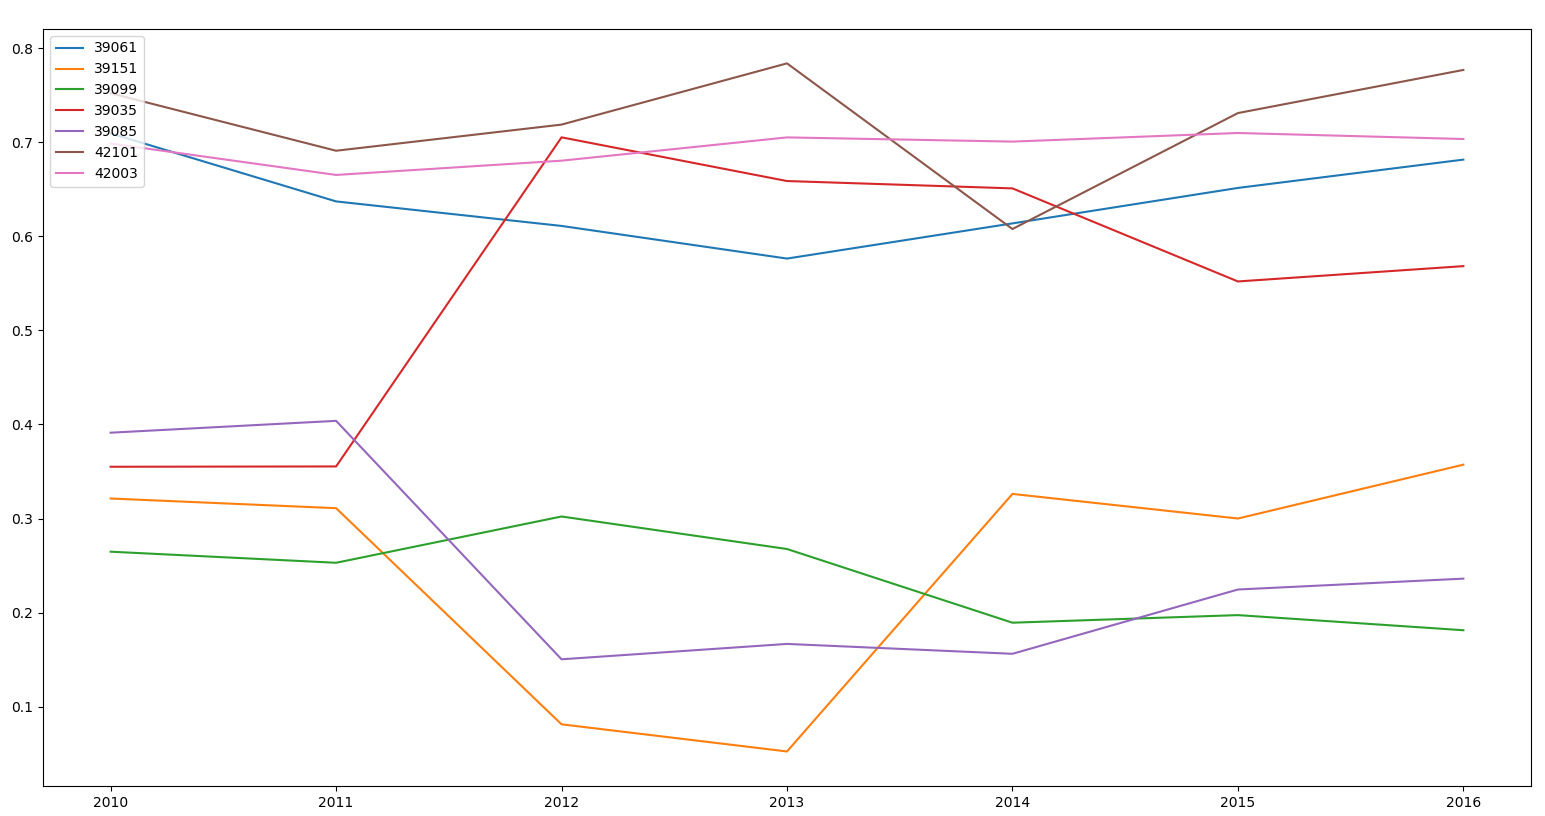
\includegraphics[width=0.6\linewidth]{004}
	\caption{$\lambda$ for the Main Sources of Opioids in General over Time}
\end{figure}

We computed $\lambda$ for the seven Main Sources during 2010-2016(see Figure 2). In order to eliminate the negative effect that a steep variation might cause, we calculate $\overline{\lambda_i}$, which is the average $\lambda$ for the $i_{th}$ Main Source through 2010-2016:

\begin{table}[H]
	\centering
\begin{tabular}{|c|c|c|c|c|c|c|c|}
	\hline
	\rowcolor[HTML]{656565} 
	{\color[HTML]{FFFFFF} \textbf{SOURCE(FIPS Code)}} &{\color[HTML]{FFFFFF} \textbf{39061}} & {\color[HTML]{FFFFFF} \textbf{39151}} & {\color[HTML]{FFFFFF} \textbf{39099}}  & {\color[HTML]{FFFFFF} \textbf{39035}} & {\color[HTML]{FFFFFF} \textbf{39085}} & {\color[HTML]{FFFFFF} \textbf{42101}}  & {\color[HTML]{FFFFFF} \textbf{42003}}\\ \hline
	$\overline{\lambda}$ & 0.6401 & 0.2499 & 0.2365 & 0.5492 & 0.2470 & 0.7231 & 0.6948 \\ \hline
\end{tabular}
\centering
\caption{$\overline{\lambda_i}$ for the Seven Main Sources}
\end{table}

As we can see in the table above, the $\overline{\lambda_i}$ obviously vary among the Main Sources. We have
\begin{equation}
\hat{\lambda}=\frac{\sum_{t=1}^{7}\overline{\lambda_i}}{7}=0.4773
\end{equation}
which indicates the average level of $\overline{\lambda_i}$, then we compute the difference of each $\overline{\lambda_i}$ from average.
\begin{equation}
\Delta \overline{\lambda_i} = \overline{\lambda_i} - \hat{\lambda}
\end{equation}
Our purpose here is to analyze which socio-economic factors contributed to such differences.

\subsection{Prior Knowledge}
The ACS dataset provided more than five hundred possible factors, so feature extraction is obviously needed. 

A series of hypothesis have been developed to explain the socio-economic factors related to opioid use. Basing on statistics summarized by the American Addiction Center and other institutes\cite{10}\cite{11}, we obtain the following information:
\begin{itemize}
	\item \textbf{EDUCATION.} College graduates aged 26 or older battled opioid addiction at lower rates than those who did not graduate from high school or those who didn’t finish college.
	\item \textbf{LONELINESS.} Those who live alone cope with opioid addiction more than those who don't.
	\item \textbf{DISABILITY.} Those with a disability are more likely to be treated with opiods and thus more likely to become addicted.
	\item \textbf{GENDER/RACE.} Contradictory reports exist on the influence of gender and entity/race on obtaining opioid addiction. 
	\item \textbf{POVERTY/UNEMPLOYMENT/FAMILY HISTORY.} Poverty, unemployment and family history are known risk factors of opioid misuse.
\end{itemize}


\begin{comment}
he above prior knowledge imply that education, loneliness, poverty, unemployment and family addiction history are the most influential factors. Contradicting reports regarding gender and entity factors allow us to assume that they play a minor part in opioid use.

Correspondingly, in the dataset, we choose \textit{\bfseries HC03\_VC85}(low educational background), \textit{\bfseries HC03\_VC14}(Nonfamily households - Householder living alone) and \textit{\bfseries HC01\_VC103}(DISABILITY STATUS OF THE CIVILIAN NONINSTITUTIONALIZED POPULATION - Total Civilian Noninstitutionalized Population). Let them be $Y_1$, $Y_2$ and $Y_3$ Further investigation showed that \textit{\bfseries HC01\_VC103} and all other disability-relevant factors were missing and therefore removed in the data cleansing proceidure. Therefore, we attempt to obtain $\lambda$ through linear regression by fitting
\begin{equation}
\lambda = \beta_1 Y_1 + \beta_2 Y_2
\end{equation}
\subsubsection{Linear Regression}
\end{comment}



%-------------------------------------

\subsection{Feature Extraction via LASSO}
We do not rely directly on prior knowledge to extract features related to $\lambda$. In order to derive useful information from the dataset, we use the LASSO method to roughly observe how each factor contributes to $\lambda$. 

Suppose that there are $N$ counties in the dataset, and each of these counties consists of $p$ covariates(i.e. socio-economic factors). We map these covariates to the corresponding total opioid use. In otherwords, the total opioid use is denoted as the \textbf{ \itshape outcome}. Let $y_i$ be the outcome(i.e. $F_i(x,y)$ in this context) and $x_i = (x_1, x_2, \cdots, x_p)^T$ be the covariate vector for the $i_{th}$ case.

To guarantee the reliability of the data, we removed all margin errors and some other redundant features including ANCESTRY, LANGUAGE, YEAR OF ENTRY and PLACE OF BIRTH. More details were discussed in section 3, Addressing Missing Data.

The LASSO estimate is defined by\cite{7}
\begin{equation}
\hat{\omega}_{LASSO}=
\arg\min_{\omega} \sum_{i=1}^{N}(y_i - x_i^T\omega)^2 + \theta||\omega||_1
\end{equation}

subject to
\begin{equation}
 \sum_{j=1}^{p}|\omega_j|\leq t
\end{equation}

Here, $t$ determines the level of regularization, and $\omega$ the weight. We fit the model using the coordinate descent algorithm. \cite{6}

We set the penalty factor $\theta$ to 1 to maximize the reduction in dimensions and extract the most valuble and relevant feature correlated with opioid use. The LASSO result of five most influential features and their weights is shown in Table 11.

\begin{table}[H]
	\centering
	\begin{tabular}{|l|l|}
		\hline
		\rowcolor[HTML]{656565} 
		{\color[HTML]{FFFFFF} \textbf{FEATURE}} & {\color[HTML]{FFFFFF} \textbf{WEIGHT}} \\ \hline
		
		Estimate; SCHOOL ENROLLMENT - 	&2083.42 \\ 
		High school (grades 9-12) & \\ \hline
		
		Estimate; HOUSEHOLDS BY TYPE - 	& -1803.94 \\
		Family households (families) - Married-couple family & \\ \hline
		Estimate; HOUSEHOLDS BY TYPE -  &	-1580.07  \\ Households with one or more people under 18 years &\\ \hline
		Estimate; EDUCATIONAL ATTAINMENT - 	& 821.73 \\ 
		9th to 12th grade, no diploma & \\ \hline
		Estimate; HOUSEHOLDS BY TYPE - & 	800.73 \\
		Nonfamily households - Householder living alone & \\ \hline
		
	\end{tabular}
	\centering
	\caption{LASSO Results}
\end{table}

We only use LASSO as a reference to help us extract the possible influential factors, instead of directly applying the weights as the final result. From Table 11 we can conclude that
\begin{enumerate}
	\item Lower educational backgound may lead to opioid use.
	\item Whether or not one lives alone relates to the possibility of opioid addiction. Family households(married/with children) may help prevent opioid usage. On the contrary, nonfamily households where householders live alone are more likely to fall victim to drugs.
\end{enumerate}

\subsection{Comparison Between Prior Knowledge and LASSO Results}
Based on reliable prior knowledge, those with a disability are more likely to use/misuse opioids. Even though there are features concerning disability in our dataset, vast amount of information is missing(we dealt with this problem in Data Processing, Section 3). 

As for possible influential factors like poverty, unemployment and family history, they are unanalyzable since no such data appeared in our dataset.

Contradicting hypothesis exist concerning the influence of gender and race on opioid usage, so we neglect these factors in our model.

To sum up, we emphasize on \textbf{EDUCATION} and \textbf{LONELINESS}. 

\begin{itemize}
\item \textbf{Education.}
We combine feature \textit{Percent; EDUCATIONAL ATTAINMENT - Less than 9th grade} and \textit{Percent; EDUCATIONAL ATTAINMENT - 9th to 12th grade, no diploma} into one single feature named \textit{Percent; EDUCATIONAL ATTAINMENT - Less than 12th grade, no diploma}.

\item \textbf{Loneliness.}
We could consider features which are positively or negatively correlated with opioid use at the same time, but this might affect the independence between features. Thus we chose the positively correlated feature \textit{Percent; HOUSEHOLDS BY TYPE - Nonfamily households - Householdgger living alone} to characterize loneliness.
\end{itemize}

\subsection{Regression Analysis}
% Next, we examine how education and loneliness contribute to $\lambda$ through linear regression.


When appling the LASSO method, we choose $F$ as the training target. $F$ is a digital value, so all features correlated with it are estimated digital values. However, when we take into account of the fact that $\lambda$ is defined by proportion, it seems more adequate for us to choose percentages which makes sense both in magnitude and actual meaning.


Our target is $\Delta \overline{\lambda_i}$. We apply similar operations on each feature, and denote them as $\Delta \overline{y_{1i}}$ and  $\Delta \overline{y_{2i}}$. Before attempting to conduct regression, we visualize the relationship between $\Delta \overline{\lambda_i}$, $\Delta \overline{y_{1i}}$ and  $\Delta \overline{y_{2i}}$.
\begin{figure}[H]
	\centering
	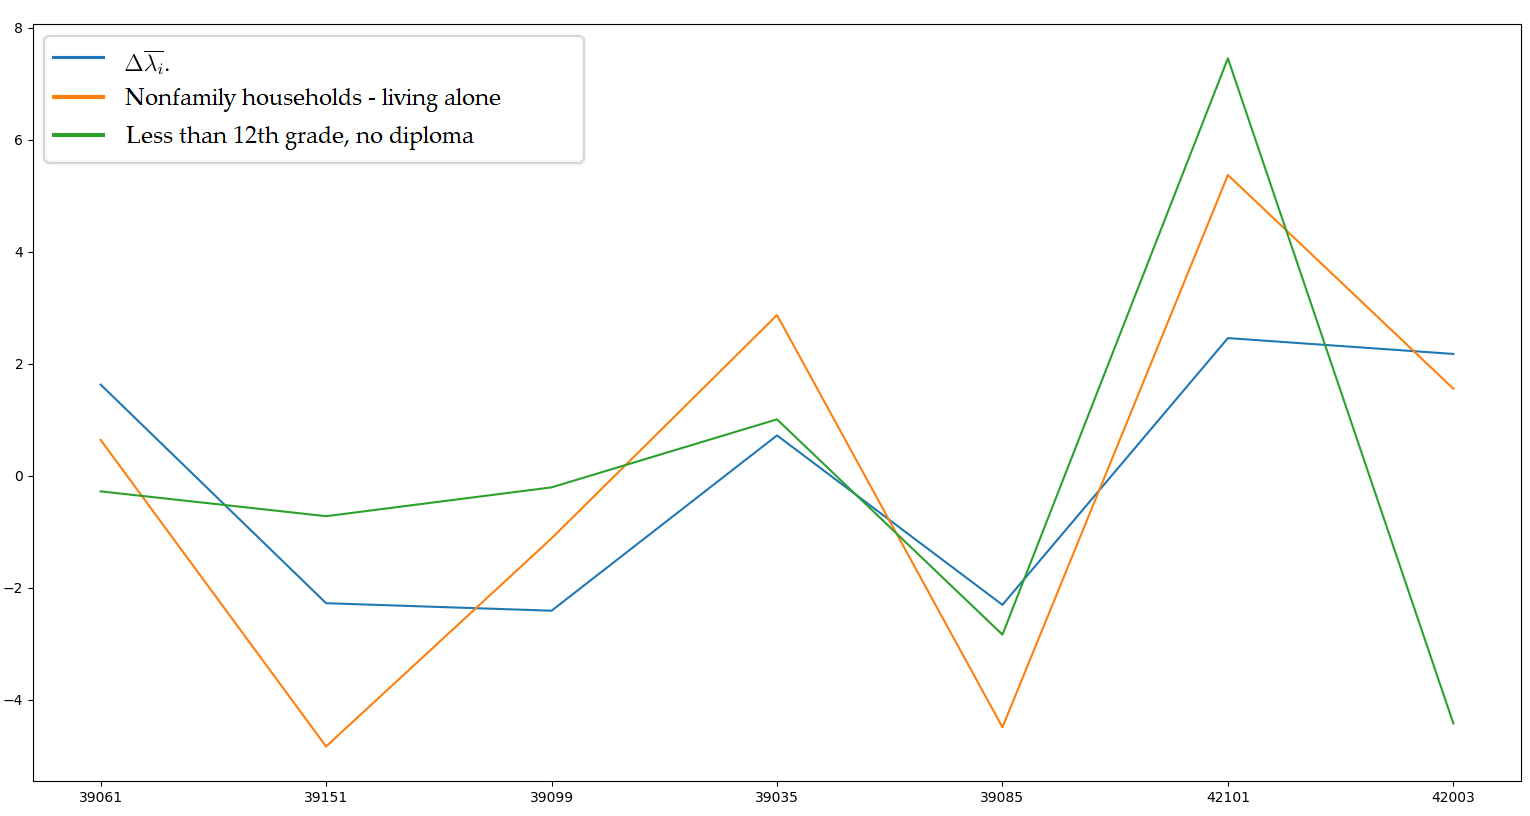
\includegraphics[width=0.7\linewidth]{005}
	\caption{the relationship between $\Delta \overline{\lambda_i}$, $\Delta \overline{y_{1i}}$ and  $\Delta \overline{y_{2i}}$}
\end{figure}

The consistency of the three attributes shown in the figure powerfully corroborated that $\Delta \overline{\lambda_i}$, $\Delta \overline{y_{1i}}$ and  $\Delta \overline{y_{2i}}$ are indeed positively correlated as we stated above. Thus, we build a linear regression model to describe their relationship as
\begin{equation}
\Delta \overline{\lambda_i} = k_1 \Delta \overline{y_{1i}} + k_2 \Delta \overline{y_{2i}} + k_3
\end{equation}

The solution to equation (20) is
\begin{equation}
\left\{
\begin{array}{l}
k_1 = 0.0193 \\
k_2 = 0.0319 \\
k_3 = -1.5340 \times 10^{-16} \\
\end{array}
\right.
\end{equation}
with coefficient of determination
\begin{equation}
R^2 = 0.9038
\end{equation} 

In the same way, we can also obtain the relationship between $\lambda_i$, $y_{1i}$ and $y_{2i}$. 

\begin{equation}
\lambda_i = k_4 y_{1i}+ k_5 y_{2i} + k_6
\end{equation}

with the solution

\begin{equation}
\left\{
\begin{array}{l}
k_4 = 0.0193 \\
k_5 = 0.0319 \\
k_6 = -0.9004 \\
\end{array}
\right.
\end{equation}

In fact, mathematically, the only difference between equation (21) and (24) is their intercepts.
Equation (24) describes how socio-economic factors affect our Opioid Spread Model from a quantitative point of view. When the details of opioid amount is not available, we would still be able to estimate the Sources' $\lambda$ through socio-economic factors.


